\documentclass[12pt, letterpaper]{article}
\usepackage{amsmath}
\usepackage{amsthm}
\usepackage{amssymb}
\usepackage[parfill]{parskip}
\usepackage{listings}
\usepackage{xcolor}
\usepackage{hyperref}
\usepackage{floatrow}
\usepackage{url}
\usepackage{graphicx}
\usepackage{multirow}
\usepackage{multicol}
\usepackage{float}
\usepackage{subcaption}
\usepackage{chemfig}
\usepackage{modiagram}
\usepackage{tikz}
\usetikzlibrary{positioning}

\lstset{
    frameround=fttt,
    language=[LaTeX]TeX,
    numbers=left,
    breaklines=true,
    delim        = [s][\color{red!50!black}]{$}{$},
    moredelim=[s][\color{red!50!black}]{\\[}{\\]},
    moredelim=[s][\color{red!50!black}]{$$}{$$},
    keywordstyle=\color{blue}\bfseries, 
    %basicstyle=\ttfamily\color{red},
    numberstyle=\tiny\color{gray},
    commentstyle=\color{green!30!black},
    stringstyle = \color{violet}
    }
    
\renewenvironment{boxed}
    {\begin{center}
    \begin{tabular}{|p{0.9\textwidth}|}
    \hline\\
    }
    { 
    \\\\\hline
    \end{tabular} 
    \end{center}
	}
	
	\begin{document}

	\title{\vspace{-2em}Advanced \LaTeX{}}
	\date{July 18, 2020}
	\author{Rwitaban Goswami and Mihir Vahanwala}
	\maketitle
	
	\tableofcontents
	
	\newpage
	\section{Introduction}
	Now that you get the hang of \LaTeX{} more or less, you will be able to do fine and apply your \LaTeX{} knowledge wherever required. But there still are some advanced things left to cover in \LaTeX{}. This week we will be briefly going over the basics of some advanced \LaTeX{} and how to proceed further.

	\section{Some other document classes}
	Till now you have only written in \verb!\documentclass{article}! exclusively. But there is a whole world out there regarding other document types, and we will cover a few of those
	\subsection{Beamer}
	Ever wondered how the MA105 slides were made? Why do they all look so uniform (and bland)? They are made using the Beamer class. While they look bland, they are dead easy and fast to generate, and are easily customizable.

	\subsubsection{Basics}
	To use beamer you need, obviously, \verb!\documentclass{beamer}! at the top of your preamble.

	A minimal working example looks like this:

	\begin{lstlisting}
\documentclass{beamer}

\usepackage{lipsum}
\usepackage[utf8]{inputenc}


%Information to be included in the title page:
\title{Beamer Introduction}
\author{Rwitaban Goswami}
\institute{IIT Bombay}
\date{18 July, 2020}



\begin{document}

\frame{\titlepage}

\begin{frame}
\frametitle{First Frame}
\lipsum[1]
\end{frame}

\end{document}
	\end{lstlisting}

	This generates the following two slides:
	\begin{figure}[ht]
		\centering
		\begin{subfigure}{0.48\textwidth}
			\includegraphics[width=\linewidth]{beamer1ppt1.png}
			\caption{Slide 1}
		\end{subfigure}
		\begin{subfigure}{0.48\textwidth}
			\includegraphics[width=\linewidth]{beamer1ppt2.png}
			\caption{Slide 2}
		\end{subfigure}
	\end{figure}

	Slides are analogous to frames in Beamer. To add new slides you need to add \verb!\begin{frame}!, and give it an appropriate title with \verb!\frametitle{}!

	But it is not necessary that each frame will produce one slide. Each frame may produce multiple pages of pdf.  For example, a frame with several bullet points can be set up to produce a new slide to reveal each consecutive bullet point.

	\subsubsection{Better titles}
	You can setup more comprehensive titles in Beamer.
	\begin{lstlisting}
\title[About Beamer]
{About the Beamer class in presentation making}

\subtitle{Beamer Intro}

\author[Rwitaban, Goswami]
{R.~Goswami\inst{1} \and M.~Vahanwala\inst{2}}

\institute[IITB]
{
  \inst{1}%
  Learner's Space instructor\\
  IIT Bombay
  \and
  \inst{2}%
  Learner's Space instructor\\
  IIT Bombay
}

\date[LS\LaTeX{}]
{Learner's Space \LaTeX{}, 18 July 2020}

\logo{\includegraphics[height=1.5cm]{ugac.jpg}}
	\end{lstlisting}
	This generates the following title:
	\begin{figure}[ht]
		\centering
		\begin{subfigure}{0.48\textwidth}
			\includegraphics[width=\linewidth]{beamer2ppt1.png}
			\caption{Slide 1}
		\end{subfigure}
	\end{figure}

	\subsubsection{TOC}
	You can even have a frame with a table of contents
	\begin{lstlisting}
\begin{frame}
	\frametitle{Table of Contents}
	\tableofcontents
\end{frame}
	\end{lstlisting}
	This generates:
	\begin{figure}[ht]
		\centering
		\begin{subfigure}{0.48\textwidth}
			\includegraphics[width=\linewidth]{beamer3ppt1.png}
			\caption{Slide 1}
		\end{subfigure}
	\end{figure}
	Keep in mind that frames are automatically not included in the TOC, the same rules as article class apply, and sections appear in the TOC

	\subsubsection{Effects}
	As we mentioned earlier, one frame may contribute to several slides. This is achieved through effects, or slideshows.
	\begin{lstlisting}
\begin{frame}
	\frametitle{Second Frame}
	This is a text in second frame. \pause
	For the sake of showing an example.
	
	\begin{itemize}
		\item<1-> Text visible on slide 1
		\item<2-> Text visible on slide 2
		\item<3> Text visible on slide 3
		\item<4-> Text visible on slide 4
	\end{itemize}
	
\end{frame}
	\end{lstlisting}
	This single frame generates 4 slides:
	\begin{figure}[ht]
		\centering
		\begin{subfigure}{0.48\textwidth}
			\includegraphics[width=\linewidth]{beamer4ppt1.png}
			\caption{Slide 1}
		\end{subfigure}
		\begin{subfigure}{0.48\textwidth}
			\includegraphics[width=\linewidth]{beamer4ppt2.png}
			\caption{Slide 2}
		\end{subfigure}
		\begin{subfigure}{0.48\textwidth}
			\includegraphics[width=\linewidth]{beamer4ppt3.png}
			\caption{Slide 3}
		\end{subfigure}
		\begin{subfigure}{0.48\textwidth}
			\includegraphics[width=\linewidth]{beamer4ppt4.png}
			\caption{Slide 4}
		\end{subfigure}
	\end{figure}

	As you can see, \verb!\item<1->! means it will be on every slide from 1 and till end of the frame. \verb!\item<3>! will mean it will be visible only on slide 3.

	You can also insert the \verb!\pause! command in between text \textit{outside} the itemize environment to generate a similar effect.

	\subsubsection{Themes}
	You can use premade themes for your slides. For example, just write \\ \verb!\usetheme{Madrid}! in your preamble to get this.
	\begin{figure}[ht]
		\centering
		\begin{subfigure}{0.48\textwidth}
			\includegraphics[width=\linewidth]{beamer5ppt1.png}
			\caption{Slide 1}
		\end{subfigure}
	\end{figure}
	Looks familiar?
	\subsubsection{Further}
	We cannot possibly even think of showing you all the commands there are in the beamer class, neither do we need to. You can use the references we have provided, search the internet, or look at the documentation to get the command and its syntax as you need.

	Other classes which are extremely useful which you can read about are:
	\begin{itemize}
		\item PowerDot (For more powerful professional looking ppts)
		\item Poster (For making highly customizable posters)
	\end{itemize}

	\section{Custom classes and packages}
	\subsection{What are classes and packages really?}
	Till now we have assumed that whatever command we want to include, we can simply add \verb!\usepackage{}! in your preamble and it will work like magic! What if we want to create our own? What if we have written a few very handy \LaTeX{} macros, and we want to package them into a package, and we can \verb!\usepackage{}! that wherever we want to?

	In essence, the default formatting in LATEX documents is determined by the class used by that document. This default look can be changed and more functionalities can be added by means of a package. The class file names have the .cls extension, the package file names have the .sty extension.

	\subsubsection{Writing your own package}
	The first thing to do before coding a new package is to determine whether you really need a new package or not. It's recommended to search on CTAN (Comprehensive TEX Archive Network) \url{https://ctan.org/ctan-portal/search/} and see if someone already created something similar to what you need.

	\subsubsection{General Structure}
	\begin{description}
		\item[Identification] The file declares itself as a package written with the \LaTeXe{} syntax.
		\item[Preliminary declarations] Here the external packages needed are imported. \\ Also in this part of the file the commands and definitions needed by\\ the declared options are coded.
		\item[Options] The package declares and processes the options.
		\item[More declarations] The main body of the package. Almost everything a package does is defined here. 
	\end{description}

	\subsubsection{Identification}
	There are two simple commands that all packages must have:
	\begin{lstlisting}
\NeedsTeXFormat{LaTeX2e}
\ProvidesPackage{examplepackage}[2014/08/24 Example LaTeX package]
	\end{lstlisting}

	The command \verb!\NeedsTeXFormat{LaTeX2e}! sets the \LaTeX{} version for the package to work. Additionally, a date can be added within brackets to specify the minimal release date required.

	The command \verb!ProvidesPackage{examplepackage}[...]! identifies this package as examplepackage and, inside the brackets, the release date and some additional information is included. The date should be in the form YYYY/MM/DD

	\subsubsection{Preliminary declarations}
	Most of the packages extend and customize existing ones, and also need some external packages to work. Below, some more code is added to the sample package ``examplepackage.st''.

	\begin{lstlisting}
\RequirePackage{imakeidx}
\RequirePackage{xstring}
\RequirePackage{xcolor}
\definecolor{greycolour}{HTML}{525252}
\definecolor{sharelatexcolour}{HTML}{882B21}
\definecolor{mybluecolour}{HTML}{394773}
\newcommand{\wordcolour}{greycolour}
	\end{lstlisting}

	The command \verb!\RequirePackage! is very similar to the well-known \verb!\usepackage!, adding optional parameters within brackets will also work. The only difference is that the \verb!\usepackage! can not be used before \verb!\documentclass! command. It's strongly recommended to use \verb!\RequirePackage! when writing new packages or classes.

	\subsubsection{Options}
	To allow some flexibility in the packages a few additional options are very useful. The next part in the file "examplepackage.sty" handles the parameters passed to the package-importing statement.
\begin{lstlisting}
\DeclareOption{red}{\renewcommand{\wordcolour}{sharelatexcolour}}
\DeclareOption{blue}{\renewcommand{\wordcolour}{mybluecolour}}
\DeclareOption*{\PackageWarning{examplepackage}{Unknown `\CurrentOption'}}
\ProcessOptions\relax
\end{lstlisting}

Below a description of the main commands that can handle the options passed to the package.

The command \verb!\DeclareOption{}{}! handles a given option. It takes two parameters, the first one is the name of the option and the second one is the code to execute if the option is passed.

The command \verb!\OptionNotUsed! will print a message in the compiler and the logs, the option won't be used.

The command \verb!\Declareoption*{}! handles every option not explicitly defined. It takes only one parameter, the code to execute when an unknown option is passed. In this case it will print a warning by means of the next command:

\verb!\PackageWarning{}{}!. This handles the errors which might occur in using the package. Lookup \url{https://www.overleaf.com/learn/latex/Writing_your_own_package} for a more detailed description on how to do that

\verb!\CurrentOption! stores the name of the package option being handled at a determined moment.

The command \verb!\ProcessOptions\relax! executes the code fore each option and must be inserted after all the option-handling commands were typed. There's a starred version of this command that will execute the options in the exact order specified by the calling commands.

In the example, if the options red or blue are passed to the \verb!\usepackage! command within the document, the command \verb!\wordcolor! is redefined. Both colours and the default grey colour were defined in the preliminary declarations after importing the xcolor package.

\subsubsection{More declarations}
In this part most of the commands will appear. In "examplepackage.sty".
\begin{lstlisting}
%%Numbered environment
\newcounter{example}[section]
\newenvironment{example}[1][]{\refstepcounter{example}\par\medskip
\noindent \textbf{My~environment~\theexample. #1} \rmfamily}{\medskip}

%%Important words are added to the index and printed in different colour
\newcommand{\important}[1]
{\IfSubStr{#1}{!}
    {\textcolor{\wordcolour}{\textbf{\StrBefore{#1}{!}~\StrBehind{#1}{!}}}\index{#1}}
    {\textcolor{\wordcolour}{\textbf{#1}}\index{#1}\kern-1pt}
}
\end{lstlisting}
This package defines the new environment example, and a new command \verb!\important!, that prints the words in a special colour and adds them to the index.
\subsubsection{Usage}
To use the package, the sty file must be in the same location as your tex file, or the relative/absolute path may be specified in \verb!\usepackage{}!
\subsection{Writing your own Class}
This is pretty similar to writing your own package, and we encourage you check out the steps here \url{https://www.overleaf.com/learn/latex/Writing_your_own_class}

\section{Some cool \LaTeX{} tricks}
Apart from custom classes and packages, there are some very handy packages which come into use in some very field specific usages. Some examples are given as follows. We cannot list out how to use every command in each of these packages, so we encourage you to check out more examples in the documentation or on the internet.
\subsection{Chemistry formulae}
There are a few \LaTeX packages to create chemistry formulae: chemfig, ochem, streetex, and xymtex. The most intuitive is probably the chemfig package.
\subsubsection{Introduction}
Drawing a molecule consists mainly of connecting groups of atoms with lines. Simple linear formulas can be easily drawn with chemfig, \verb!\chemfig{O=H}! generates \chemfig{O=H}. The command \verb!\chemfig{O=H}! the draws the molecule. The symbol = determines the type of bond.
\subsubsection{Angles}
There are several ways to define angles to draw the bonds between molecules.
\begin{lstlisting}
\chemfig{A-[1]B-[7]C}
\chemfig{A-[:50]B-[:-25]C}
\chemfig{A-[::50]B-[::-25]C}
\end{lstlisting}
\chemfig{A-[1]B-[7]C}
\chemfig{A-[:50]B-[:-25]C}
\chemfig{A-[::50]B-[::-25]C}

Each one of the three commands in the example above uses a different method to determine the angle between bonds.

\begin{description}
	\item[default units] In the command \verb!\chemfig{A-[1]B-[7]C}! the parameters inside brackets set the angle in special units, each unit equals 45$^\circ$. Hence in the example the angles are 45$^circ$ and 315$^\circ$.
	\item[absolute units] The angles can be set in absolute units, in the command \verb!\chemfig{A-[:50]B-[:-25]C}! the parameter inside the brackets represent the angle, in degrees, measured from the horizontal baseline. Negative angles are allowed.
	\item[relative angles] In the third example \verb!\chemfig{A-[::50]B-[::-25]C}! the angles are measured from the previous bond, instead of the baseline.
\end{description}
\subsubsection{Rings and Branches}
You can even draw rings or branches using this package
\begin{lstlisting}
\chemfig{A*5(-B=C-D-E=)}
\chemfig{A*5(-B=C-D)}
\chemfig{H-C(-[2]H)(-[6]H)-C(=[1]O)-[7]H}
\chemfig{A*6(-B=C(-CH_3)-D-E-F(=G)=)}
\end{lstlisting}
\chemfig{A*5(-B=C-D-E=)}
\chemfig{A*5(-B=C-D)}
\chemfig{H-C(-[2]H)(-[6]H)-C(=[1]O)-[7]H}
\chemfig{A*6(-B=C(-CH_3)-D-E-F(=G)=)}

\subsubsection{Formatting}
You can customize the formatting using several parameters. Check \url{https://www.overleaf.com/learn/latex/Chemistry_formulae} for a reference

\subsection{MO Diagrams}
\subsubsection{Introduction}
Molecular diagrams are created using the package modiagram
\begin{lstlisting}
\begin{MOdiagram}
	\atom{left}{1s, 2s, 2p}
\end{MOdiagram}
\end{lstlisting}
\begin{center}
    \begin{MOdiagram}
    	\atom{left}{1s, 2s, 2p}
    \end{MOdiagram}
\end{center}

The basic command to draw MO diagrams is \verb!\atom!. This command has two parameter in the example:

\begin{description}
    \item[left] The alignment of the atom.
    \item[1s, 2s, 2p] The energy sub-levels to be drawn.
\end{description}

You can pass some extra information about the atomic orbitals to the command presented in the introductory example.

\begin{lstlisting}
\begin{MOdiagram}
 \atom{right}{
    1s = { 0; pair} ,
    2s = { 1; pair} ,
    2p = {1.5; up, down }
 }

 \atom{left}{
    1s = { 0; pair} ,
    2s = { 1; pair} ,
    2p = {1.5; up, down }
 }
\end{MOdiagram}
\end{lstlisting}
\begin{center}
    \begin{MOdiagram}
     \atom{right}{
        1s = { 0; pair} ,
        2s = { 1; pair} ,
        2p = {1.5; up, down }
     }
    
     \atom{left}{
        1s = { 0; pair} ,
        2s = { 1; pair} ,
        2p = {1.5; up, down }
     }
    \end{MOdiagram}
\end{center}

The generic syntax to create atoms is: \verb!1s = {energy; specifications}!
\subsubsection{Molecules}
The syntax for molecules is very similar to that of the \verb!\atom!. The energy sub-levels 1s, 2s and 2p become 1sMO, 2sMO and 2pMO respectively.

\begin{lstlisting}
\begin{MOdiagram}
 \atom{left}{1s}
 \atom{right}{1s={;up}}
 \molecule{
    1sMO={0.75;pair,up}
  }
\end{MOdiagram}
\end{lstlisting}
\begin{center}
    \begin{MOdiagram}
     \atom{left}{1s}
     \atom{right}{1s={;up}}
     \molecule{
        1sMO={0.75;pair,up}
      }
\end{MOdiagram}
\end{center}

\subsection{Diagrams}
One of the most extensive and useful packages in \LaTeX{} is probably the Tikz package, used to draw any kinds of diagrams imaginable. We will just show you a few possibilites that tikz opens up for you.
\subsubsection{Introduction}
First, you declare a tikzpicture environment, before this you must include the line \verb!\usepackage{tikz}! in the preamble of your document.

\begin{lstlisting}
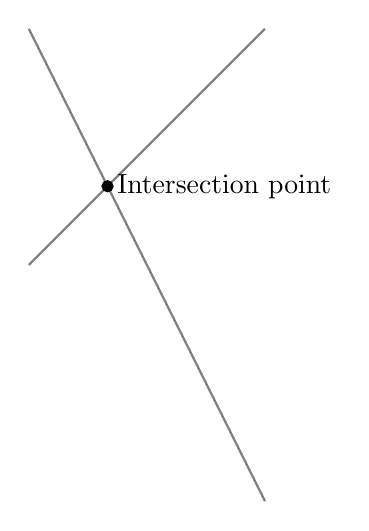
\begin{tikzpicture}
    \draw[gray, thick] (-1,2) -- (2,-4);
    \draw[gray, thick] (-1,-1) -- (2,2);
    \filldraw[black] (0,0) circle (2pt) node[anchor=west] {Intersection point};
\end{tikzpicture}
\end{lstlisting}
\begin{center}
    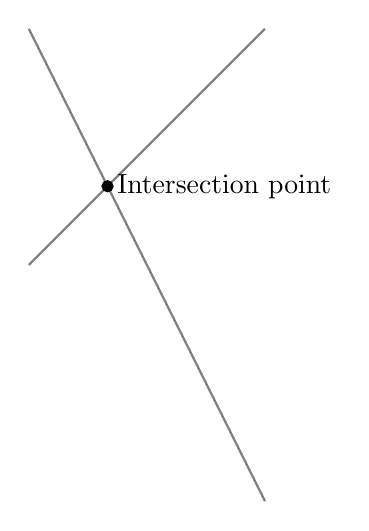
\begin{tikzpicture}
        \draw[gray, thick] (-1,2) -- (2,-4);
        \draw[gray, thick] (-1,-1) -- (2,2);
        \filldraw[black] (0,0) circle (2pt) node[anchor=west] {Intersection point};
    \end{tikzpicture}
\end{center}

See how powerful it is? Even with a few commands you can make extremely flexible graphics.

\subsubsection{Basic elements: points, lines and paths}
In this section is explained how to create basic graphic elements. These elements can be combined to create more elaborated figures.
\begin{lstlisting}
\begin{tikzpicture}

    \draw (-2,0) -- (2,0);
    \filldraw [gray] (0,0) circle (2pt);
    \draw (-2,-2) .. controls (0,0) .. (2,-2);
    \draw (-2,2) .. controls (-1,0) and (1,0) .. (2,2);

\end{tikzpicture}

\end{lstlisting}
\begin{center}
    \begin{tikzpicture}
        \draw (-2,0) -- (2,0);
        \filldraw [gray] (0,0) circle (2pt);
        \draw (-2,-2) .. controls (0,0) .. (2,-2);
        \draw (-2,2) .. controls (-1,0) and (1,0) .. (2,2);
    \end{tikzpicture}
\end{center}

There are three basic commands in this example:

\verb!\draw (-2,0) -- (2,0);!
This defines a line whose endpoint are (-2,0) and (2,0).
\verb!\filldraw [gray] (0,0) circle (2pt);!
The point is created as a very small gray circle centred at (0,0) and whose radius is (2pt). The \verb!\filldraw! command is used in to draw elements and fill them with some specific colour. See the next section for more examples.
\verb!\draw (-2,2) .. controls (-1,0) and (1,0) .. (2,2);!
Draws a Bézier curve, is a bit tricky at first. There are 4 points defining it: (-2,2) and (2,2) are its endpoints, (-1,0) and (1,0) are control points (can be equal) that determine 'how curved' it is. You can think of these two points as "attractor points".

Note that all tikz commands end in a semicolon
\subsubsection{Basic geometric shapes: Circles, ellipses and polygons}
Geometric figures can be made up from simpler elements or created by an special command. Let's start with circles, ellipses and arcs.
\begin{lstlisting}
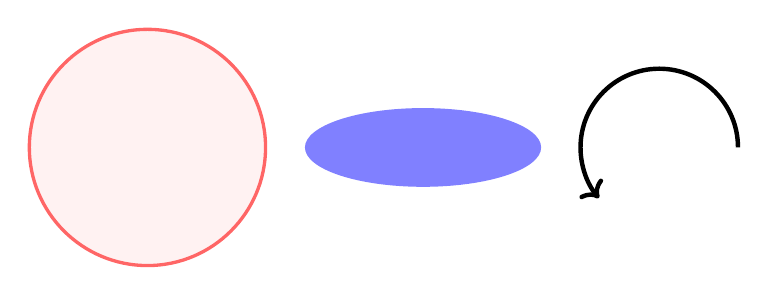
\begin{tikzpicture}
    \filldraw[color=red!60, fill=red!5, very thick](-1,0) circle (1.5);
    \fill[blue!50] (2.5,0) ellipse (1.5 and 0.5);
    \draw[ultra thick, ->] (6.5,0) arc (0:220:1);
\end{tikzpicture}
\end{lstlisting}

\begin{center}
    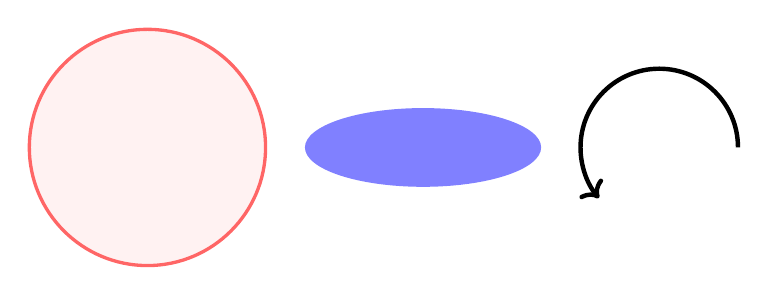
\begin{tikzpicture}
        \filldraw[color=red!60, fill=red!5, very thick](-1,0) circle (1.5);
        \fill[blue!50] (2.5,0) ellipse (1.5 and 0.5);
        \draw[ultra thick, ->] (6.5,0) arc (0:220:1);
    \end{tikzpicture}
\end{center}

\subsubsection{Nodes}
The nodes are probably the most versatile elements in Tikz. We've already used one node in the introduction to add some text to the figure. In the next example nodes will be used to create a diagram.
\begin{lstlisting}
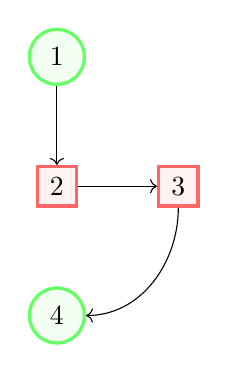
\begin{tikzpicture}[
    roundnode/.style={circle, draw=green!60, fill=green!5, very thick, minimum size=7mm},
    squarednode/.style={rectangle, draw=red!60, fill=red!5, very thick, minimum size=5mm},
    ]
    %Nodes
    \node[squarednode]      (maintopic)                              {2};
    \node[roundnode]        (uppercircle)       [above=of maintopic] {1};
    \node[squarednode]      (rightsquare)       [right=of maintopic] {3};
    \node[roundnode]        (lowercircle)       [below=of maintopic] {4};
    
    %Lines
    \draw[->] (uppercircle.south) -- (maintopic.north);
    \draw[->] (maintopic.east) -- (rightsquare.west);
    \draw[->] (rightsquare.south) .. controls +(down:7mm) and +(right:7mm) .. (lowercircle.east);
\end{tikzpicture}
\end{lstlisting}

\begin{center}
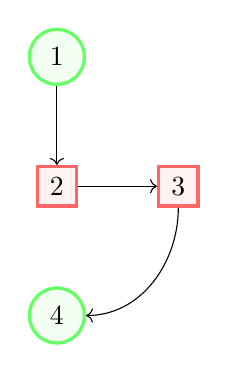
\begin{tikzpicture}[
    roundnode/.style={circle, draw=green!60, fill=green!5, very thick, minimum size=7mm},
    squarednode/.style={rectangle, draw=red!60, fill=red!5, very thick, minimum size=5mm},
    ]
    %Nodes
    \node[squarednode]      (maintopic)                              {2};
    \node[roundnode]        (uppercircle)       [above=of maintopic] {1};
    \node[squarednode]      (rightsquare)       [right=of maintopic] {3};
    \node[roundnode]        (lowercircle)       [below=of maintopic] {4};
    
    %Lines
    \draw[->] (uppercircle.south) -- (maintopic.north);
    \draw[->] (maintopic.east) -- (rightsquare.west);
    \draw[->] (rightsquare.south) .. controls +(down:7mm) and +(right:7mm) .. (lowercircle.east);
\end{tikzpicture}
\end{center}

There are essentially three commands in this figure: A node definition, a node declaration and lines that join two nodes.

\verb|roundnode/.style={circle, draw=green!60,|\\
\verb|fill=green!5, very thick, minimum size=7mm}|\\
Passed as a parameter to the tikzpicture environment defines a node that will be referred as roundnode, this node will be a circle whose outer ring will be green!60 and will be coloured with green!5, the stroke will be very thick and its minimum size is 7mm. The line below this defines a second rectangle-shaped node called squarednode with similar parameters.

\verb!\node[squarednode] (maintopic) {2};!\\
This will create a squarednode, as defined in the previous command. This node will have an id, maintopic and will contain the number 2, if you leave an empty space inside the braces no text will be displayed.

\verb![above=of maintopic]!\\
Notice that all but the first node have an additional parameter, this parameter determines its position relative to other node. For instance [above=of maintopic] means that this node should appear above the node named maintopic. For this positioning system to work you have to add \verb!\usetikzlibrary{positioning}! to your preamble. Without the positioning library, you can use the syntax above of=maintopic instead, but the positioning syntax is more flexible and powerful: you can extend it to write above=3cm of maintopic i.e. control the actual distance from maintopic.

\verb!\draw[->] (uppercircle.south) -- (maintopic.north);!\\
An arrow-like straight line will be drawn. The syntax has been already explained at the basic elements section. The only thing special is the manner we write the endpoints of the line, by referencing a node (this is why we named them) and a position relative to the node.
\subsection{Further}
There are a lot more packages out there, here are a few we encourage you to go check out (some of them are requirements for completing the assignment)
\begin{description}
    \item[tikz-3dplot] Like tikz but lets you draw in 3D!
    \item[skak] Useful for drawing chess notation as well as chessboards
    \item[knittingpatterns] A useful package to make your document look better by using knitting patterns to embed your paragraphs in
    \item[CircuiTikz] Versatile like tikz, has similar syntax but specializes in drawing electrical circuit diagrams
    \item[exam] Useful for typesetting exams
\end{description}
\end{document}
